%!TEX root=..\master.tex
\section{The Bell-LaPadula Security Policy}

Bell and LaPadula have devised a mathematical model intended for use in  military and governmental computer systems.
The model formalizes users accessing data and how to handle this in a secure way so confidential information cannot be leaked to a lower classification level.
The following description is based on \citet{lapadula1996secure}.

\subsection{Security}
Before we go into details about how the Bell-LaPadula (BLP) security model is applied to computer systems, we will first discuss some important concepts.

In any system we will have a set of objects $O$ and \subjects{} $S$.
Objects are entities that can somehow be manipulated by \subjects{}.
\Subjects{} are processes or programs in execution that represent a user or a group of users.

\paragraph{Classification and Clearance}
Attached to any object or \ssubject{} will be a classification or clearance respectively.
We denote the set of all classifications/clearances $C = \{C_1, C_2,\dots,C_q\}$ where $\{C_1 > C_2 > \dots > C_q\}$ holds, giving a hierarchical sequence of classifications/clearances.
This means that for any object $o \in O$ with \textit{classification} $C_i \in C$, where $C_i$ is arbitrary, any \ssubject{} $s \in S$ will need a \textit{clearance} $C_j \geq C_i$ in order to access $o$.

\paragraph{Category and Need-to-know}
In addition to classification, objects can belong to one or more categories, which can be seen as security groupings of certain objects.
Similarly, \subjects{} can have one or more need-to-know, which are the security groupings for \subjects{}.
The security categories are a set $K = \{K_1, K_2, \dots, K_r\}$ and unlike classifications/clearances there is no hierarchy of categories.
In order for \ssubject{} $s$ to access an object $o$ with \textit{category} $K_m$ and $K_n$, where $K_m$ and $K_n$ are arbitrary, $s$ must have both \textit{Need-to-know} categories $K_m$ and $K_n$.

\paragraph{Classification and category vectors}
 In the model classifications and categories are stored in vectors.
 Four functions are used for lookup in these vectors.
 $F_1$ performs a lookup in the subject classification vector, $F_2$ in the object classification vector, $F_3$ in the subject category vector and finally $F_4$ performs a lookup in the object category function.

\paragraph{Visualization}
This kind of security system can be seen as a \textit{lattice}, see \cref{blp:lattice}.
Each node represents a \emph{security level} -- i.e. a combination of classification/clearance and a set of categories.
\mikael{'security level' er noget jeg fandt på, hvordan skal vi håndtere det?}
A \ssubject{} with the clearance \emph{Top Secret} is able to access any object with the security level \emph{Top Secret} as well as all those below (\emph{Secret} and \emph{Unclassified}).
On the contrary, a \ssubject{} with clearance \emph{Unclassified} can only access objects with the security level \emph{Unclassified}.

Similarly, the category(ies) of each node limit what objects a \ssubject{} can access.
If we have a subject $s$ with clearance \emph{Top Secret} and category \emph{Crypto}, $s$ will have access to any objects with security level $(Top Secret, \{Crypto\})$ and those below.

\begin{figure}
\centering
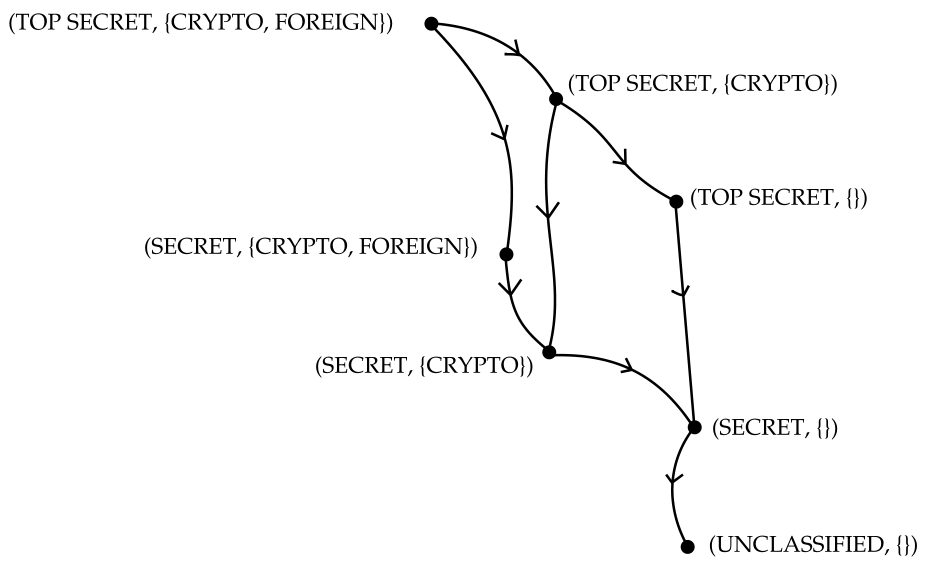
\includegraphics[width=\textwidth]{figures/blp_lattice}
\caption{A BLP lattice \cite{security_engineering_ross_anderson}}
\label{blp:lattice}
\end{figure}

\subsection{Access attributes}
The model considers four attributes for access in a complex computer system: \emph{read-only}, \emph{append}, \emph{execute} and \emph{read/write}.
In addition \emph{control access} is used to give attributes to other users.
Formally, the access attributes are defined as a set $A = \{ \underline{r}, \underline{w}, \underline{e}, \underline{a}, \underline{c} \}$, each member corresponding to the aforementioned attributes.

\paragraph{Read-only}
This attribute makes it possible to read the object but not alter it.
The classical example is a file that contains information that should not be changed.
Alternatively it could be a list containing the \principals{} in the system with their clearance levels.
A \principal{} of low clearance should be able to read this list but not change it.

\paragraph{Append}
Append describes a pure write operation.
This means that it is possible to append information to the end of a file without being able to extract information about the rest of the file.

This can also be used with a printer which appends information about what is being printed.
By doing this it is sufficient that the classification of a piece of information is matching the classification of the printer in order to prevent unauthorized personnel from reading the information.

\paragraph{Execute}
The execution attribute makes it possible to execute an executable file.
If the \principal{} does not have permission to read from or write to the file he will only be able to execute it.
Similarly the executable file can produce output that is of a higher classification level than the clearance level of the \principal{} executing it.

\paragraph{Read/write}
This attribute signifies that read and write access are both allowed.
This attribute is what is traditionally used when editing text files.

\paragraph{Control access}
The control access attribute models the notion of a \principal{} having control over a file.
Having this attribute a \principal{} can give the four attributes above to other \principals{} in the system.

\subsection{Requests and decisions}
In a computer system the \principals{} are not directly accessing objects in the system, it is processes in the system that act on behalf of the \principal{}.
In the following a user requesting access to a file will be written as a \principal{} requesting access and the response to this request a decision

\subsection{Preventing security compromise}\label{bellap:properties}
In order to ensure that data cannot be compromised the previous definitions of access attributes and requests can be utilized to formalize properties that ensure that compromise cannot occur.

\subsubsection{Security condition}
The security condition states that a \principal{} with a given clearance level is prevented from having read access to any object which is or can be a source of information with a classification level that is higher than the clearance level of the \principal{}.

Formally this can be expressed as the following:
\begin{definition}
The access matrix contains entries of the form $(s,o,x)$ where $s \in S, o \in O \text{ and } x \in A$.
Such entry satisfies the security condition relative to the classification and need-to-know vectors if and only if

\begin{itemize}
\item x is either the \emph{execute}, \emph{append} or \emph{control} access attribute, or
\item x is the \emph{write} or the \emph{read} attribute and both $f_1(s) \ge f_2(o)$ and $f_3(s) \supseteq f_4(o)$
\end{itemize}

An \emph{access matrix} is secure if every access matrix entry satisfies the security condition.

A system consists of \emph{appearances} which consists of requests and decisions that manipulate the access matrix.

A \emph{system} is a secure system if and only if every appearance of the system is secure.
\end{definition}

Seen in context of the lattice in \cref{blp:lattice}, the security condition can be seen as the disallowance of any subject $s$ from reading any objects above its security level (\textbf{no read-up}).

\subsubsection{*-property}
The *-property states that if a \principal{} has write or append access to objects and read or read/write access to some objects, then the objects which he has write or append access to must exceed or equal the objects which he has read or write access to.
This property ensures that it is impossible to leak information to a lower classification level.

The following definition expresses this formally:
\begin{definition}
Let $b(S:x,y, \dots, z)$ denote the set 

$\{O: o \in O \text{ and } [(s,o,x) \in b, (s,o,y) \in b, \dots, (s,o,z) \in b]\}$.

Here b is the set of access matrix entries of some access matrix.

\paragraph{}
\noindent{} 
A state of an access matrix satisfies the *-property if an only if for each $s \in S$ the following proposition holds.

$[b(s:w,a) \ne \emptyset \text{ and } b(s:r,w) \ne \emptyset] \implies [f_2(O_1) \ge f_2(O_2) \text{ and } f_4(O_1) \supseteq f_4(O_2) \text{ for all } O_1 \in b(s:w,a), O_2 \in b(s:r,w)]$

\paragraph{}
\noindent{} 
A system is satisfying the *-property if and only if every appearance of the system satisfies the *-property.
\end{definition}

When seeing the *-property in the context of \cref{blp:lattice}, the *-property states that it is not allowed for any subject $s$ to read any object $o_1$ and write any of this information to an object $o_2$, if $o_2$ is not above, or at the same security level as, $o_1$ (\textbf{no write-down}).
